\section{Optimal Transport}%
\label{sec:optimal-transport}

\vspace{1cm}

\begin{figure}[h]%
  \label{fig:paradise}
  \centering
  \fcolorbox{black}{white} {
    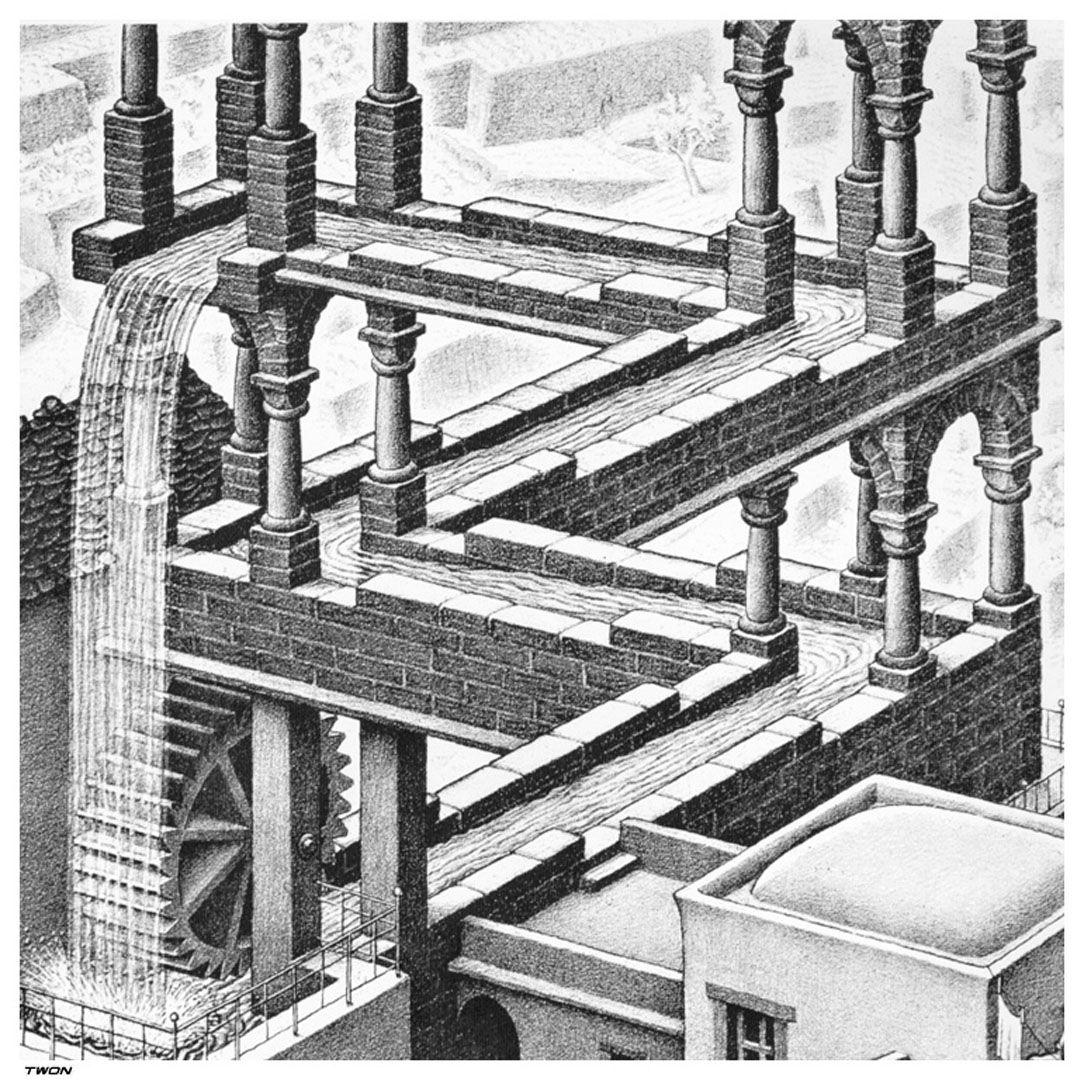
\includegraphics[width=0.3\textwidth]{escher}
  }
  \caption{M.C. Escher, ``Waterfall'', 1961.}
\end{figure}

\vspace{1cm}

\lettrine[lines=3]{\Royal~S}{ection~\ref{sec:information-theory}
  uncovered how the generator minimizes} an approximation of the
Jensen-Shannon divergence of $\pt$ and $\pg$ which the discriminator
approximated at each training step.

In this section we discuss the limitations of $\V$ as the GAN
objective function which come from the metric topology induced by the
Jensen-Shannon divergence. To this end, we provide an introduction to
some relevant concepts from topology in order to understand the
aforementioned limitations.

We also provide an introduction to optimal transport and what is
commonly referred to as the earth mover or Wasserstein distance in
order to properly cover a variant of the GAN algorithm called the
Wasserstein GAN (WGAN). The WGAN was introduced
by~\cite{ref:arjovsky-2017} from the Courant Institute of Mathematical
Sciences as an attempt to overcome certain obstacles in GAN training.

The moral of this section is the choice of distance function to
furnish a space $\&X$ with has profound consequences on properties of
continuity and therefore the ability of sequences of probability
distributions to convergence within $\&X$.

% The reason for this has to do with the topological properties
% induced by the choice of distance.

A topological space is the most general notion of a mathematical space
that allows for the definition of concepts like continuity and
convergence.  Other spaces such as manifolds and metric spaces are
specializations of topological spaces with extra structure or
constraints.  A space $\&X$ can be furnished with various different
distance functions.  The \textit{open balls} form the base for a
topology on $\&X$, which makes $\&X$ into a \textit{topological
  space}.

% \begin{definition}
%   Let $(\&X, d)$ be a metric space. An \textbf{open ball} of radius
%   $r \in \R^+$ around the point $x_0 \in \&X$ is the set
%   \begin{align}
%     \&B_r(x_0) = \left\{ x \in \&X : d(x,x_0) < r \right\}.
%   \end{align}
%   That is to say $\&B_r(x_0)$ is the set of all points in $\&X$ that
%   are not more than a distance of $r$ from $x_0$.
% \end{definition}

\begin{definition}%
  \label{def:topology1}
  Let $\&X$ be any set. A \textbf{topology} $\&T$ on $\&X$ is a
  collection of subsets of $\&X$, each called an open set, such that
  \begin{enumerate}[(i)]
  \item the empty set and the set containing all of $\&X$ are open;
  \item the intersection of finitely many open sets is an open set;
  \item the union of any collection of open sets is an open set.
  \end{enumerate} The set $\&X$ along with a topology $\&T$ on $\&X$
  is called a \textbf{topological space}.
\end{definition}

The notion of the \textit{open ball} is fundamental to the topology of
a metric space.  Useful topological definitions (useful from the
perspective of the practising statistician) can be formed from the
notion of the \textit{open ball}.

\begin{definition}%
  \label{def:open-ball}
  Let $(\&X, \&D)$ be a metric space. An \textbf{open ball} of radius
  $r \in \R^+$ around the point $x_0 \in \&X$ is the set
  \begin{align}
    \&B_r(x_0) = \left\{ x \in \&X : \&D(x,x_0) < r \right\}.
  \end{align}
  That is to say $\&B_r(x_0)$ is the set of all points in $\&X$ that
  are within $r$ distance from $x_0$.
\end{definition}

\begin{definition}%
  \label{def:topology2}
  Let $(\&X, d)$ be a metric space.  The topology generated by the
  basis of open balls
  $\&B = \{\&B_d(x, \epsilon) \mid x \in \&X, \epsilon > 0\}$ is
  called the \textbf{topology induced by} $d$ and is referred to as a
  \textbf{metric topology}.
\end{definition}

Different metrics induce different topologies which are characterized
by the quality of granularity.

\begin{theorem}%
  \label{thm:granularity}
  Let $d$ and $d^\prime$ be metrics on a set $\&X$, and let $\&T$ and
  $\&T^\prime$, be the respective topologies they induce.
  $\&T^\prime$ is \textbf{finer} than $\&T$ if and only if for each
  $x \in \&X$ and $\epsilon > 0$, there exists a $\delta > 0$ such
  that $\&B_{d^\prime}(x, \delta) \subset \&B_d(x, \epsilon)$.
\end{theorem}

\begin{definition}%
  \label{def:convergence-metric-space}
  Let $\&X$ be any finite set of events, and $\&P$ be the space of all
  probability distributions over $\&X$ with equal support. Let
  $d: \&P \times \&P \mapsto \mathbb{R}$ be a metric on this space.  A
  sequence of probability distributions ${(P_n)}_{n \in \mathbb{N}}$
  \textbf{converges} to a probability distribution $P$ if for any
  $\epsilon > 0$ there exists $N(\epsilon) \in \mathbb{N}$ such that
  $d(P_n,P) < \epsilon$ for all $n > N(\epsilon)$.
\end{definition}

The ease in which a sequence of probability distributions
${(P_n)}_{n \in \mathbb{N}}$ converges to some $P$ is determined by
the notion of distance.  The Kullback-Leibler and Jensen-Shannon
divergences induce a coarser topology than the topology induced by the
\textit{earth mover distance}. The interested reader can see the proof
of this in~\cite{ref:arjovsky-2017}.  To ease convergence, we want to
place a finer topology on $\&P \times \&P$.  A finer topology means we
can pack more open sets over $\&P \times \&P$, which makes it easier
to define a \textit{continuous map} from $\&P \times \&P$ to $\R^+$.
If a metric $d$ induces a finer topology on a space than another
metric $d^\prime$, then we say $d$ is a weaker notion of distance than
$d^\prime$.

We can think of continuity and convergence in more than one way, below
we include the relevant definitions from both the topological and
metric space points of view.

\begin{definition}%
  \label{def:continuity-metric-space}
  A function $f: \R \mapsto \R$ is \textbf{continuous} if for every
  $x_0 \in \R$, $\epsilon > 0$, there exists $\delta > 0$ such that if
  $|x - x_0| < \delta$, then $|f(x) - f(x_0)| < \epsilon$.
\end{definition}

Continuous functions between topological spaces preserve proximity,
i.e.\ a continuous function maps points that are close together in one
space to points that are close together in the other space.

\begin{definition}%
  \label{def:convergence-topological-space}
  In a topological space $(\&X, \&T)$, a sequence of points
  \textbf{converges} to $x \in \&X$ if for every neighborhood $U$ of
  $x$, there is an $N \in \mathbb{N}$ such that $x_n \in U$ for all
  $n \geq N$.
\end{definition}

The following is the topological definition of continuity. Briefly,
$f$ is continuous if the \textit{preimage} of every open set is open.

\begin{definition}%
  \label{def:pre-image}
  Given a function $f: \&X \mapsto \&Y$ and a point $y \in \&Y$,
  define $f^{-1}(y)$, the \textbf{preimage} of $y$, to be the set
  $\{x \in \&*X \mid f(x) = y\}$.  For any set $A \subset \&Y$, the
  preimage of $A$, $f^{-1}(A) = \{x \in \&X \mid f(x) \in A\}$.
\end{definition}

\begin{definition}%
  \label{def:continuity-topological-space}
  Let $\&X$ and $\&X^\prime$ be topological spaces. A function
  $f: \&X \mapsto \&X^\prime$ is \textbf{continuous} if $f^{-1}(V)$ is
  open in $\&X$ for every open set $V$ in $\&X^\prime$.
\end{definition}

The problem with the Kullback-Leibler and Jensen-Shannon divergences
is that they are strong notions of distance. Which means continuity of
the loss function may be lost under certain commonly encountered
circumstances in GAN training.

\subsection{Limitations of the Kullback-Leibler Divergence}

In~\cite{ref:arjovsky-2017}, the authors use the example of learning
parallel lines and here we present the same example. This is an
example of what happens with the Kullback-Leibler and Jensen-Shannon
divergences when we compare distributions over the same space but with
disjoint supports, see Definition \ref{def:kl-divergence} for more
information on the Kullback-Leibler divergence.

\begin{example}[Learning Parallel Lines]
  \begin{figure}[h] \centering
    \begin{tikzpicture}[scale=2,>=stealth]
      \draw[line] (-1,-0.5) rectangle (2,2);
      \draw[red, thick, ->] (0,0) -- (0,1);
      \draw[blue, thick, ->] (1,0) -- (1,1);
      \draw[dotted] (-0.8,0) -- (1.8,0) node[anchor=north east]{$x$};
      \draw[dotted] (0,-0.3) -- (0,1.8) node[anchor=north east]{$y$};
      \draw (0,0) node[anchor=north east]{$(0,z)$};
      \draw (1,0) node[anchor=north east]{$(\phi,z)$};
    \end{tikzpicture}
    \caption{Parallel Lines}%
    \label{fig:parallel-lines}
  \end{figure}%
  \label{example:learning-parallel-lines}

  Let $\&X = \R^2$ and let $p_0(z)$ be the distribution of tuples
  $(0, z) \subset \R^2, z \in [0, 1]$, i.e.\ we have a uniform
  distribution over the $y$-axis of $\R^2$ of length 1 starting at the
  origin. Let $\G(z)$ be the distribution of tuples
  $(\phi, z) \subset \R^2$ (a generative model), where $\phi$
  parameterizes the location of the distribution with respect to the
  $x$-axis. We want to train $\G(z)$ to approximate $p_0(z)$, i.e.\ we
  want $\phi \to 0$.
  \begin{enumerate}[(i)]
  \item If we use the Kullback-Leibler divergence to measure the
    distance between $p_0(z)$ and $\G(z)$ we observe the following
    discontinuity between changes in the parameter $\phi$ and the
    divergence
    \begin{align}
      \KL{p_0(z)}{\G(z)} = \E{z \sim p_0(z)}{\log{p_0(z)\over\G(z)}},
    \end{align}
    since the expectation above is taken with respect to the
    distribution over the line $(0, z)$, the line will have measure
    zero with respect to the distribution $\G(z)$. Thus
    $\KL{p_0(z)}{\G(z)} = \infty$, unless $\phi = 0$, then
    $\KL{p_0(z)}{\G(z)} = 0$. The same occurs with
    $\KL{\G(z)}{p_0(z)}$.
  \item The Jensen-Shannon divergence ends up being equally useless
    since
    \begin{align}
      \JSD{p_0(z)}{\G(z)} & = {1 \over 2} \E{z \sim p_0(z)}{\log{p_0(z)
                            \over p_m(z)}} + {1 \over 2} \E{z \sim
                            \G(z)}{\log{\G(z) \over p_m(z)}} \\
                          & = {1 \over 2} \E{z \sim p_0(z)}{\log{2}} + {1
                            \over 2} \E{z \sim \G(z)}{\log{2}} \\
                          & = \log{2},
    \end{align}
    where $p_m(z) = {p_0(z) + \G(z) \over 2}$. In the first term
    $\G(z) = 0$ because $z \sim p_0(z)$ and in the second term
    $p_0(z) = 0$ because $z \sim \G(z)$. Which is to say
    $\JSD{p_0(z)}{\G(z)} = \log{2}$, unless $\phi = 0$, in that case
    $\JSD{p_0(z)}{\G(z)} = 0$.
  \end{enumerate}
\end{example}

% The reason why this happens has something to do with topology. We
% need to relax the convergence requirements, we need to relax the
% continuity requirements.

The reason why this happens is a central topic
in~\cite{ref:arjovsky-towards-2017} and is due to the combination of
the strong notion of distance of the Jensen-Shannon divergence and the
artificially high dimensionality of most data sets.  For example, a
data set may live in $\R^n$ for some large $n$, but there may only be
variation of interest in a small number of dimensions. This is one of
the ideas motivating dimensionality reduction algorithms like PCA and
manifold learning algorithms in particular like
Isomap~\cite{ref:tenenbaum-2000}.

GANs are often used in the generation of realistic looking images. If
we consider an image to be a point in
$\&X = {[0, 255]}^{3 \times H \times W}$, the space of 8-bit RGB
images, and if we were to sample a point from this space, it would
most likely look like noise. Thus, any data set of images would
correspond to a very small subset, or \textit{data manifold}, of
$\&X$. An informal definition of a \textit{manifold} is more useful to
our discussion than a formal one. When we say \textbf{manifold}, we
mean a continuous geometrical structure with finite dimension (e.g.\ a
line, a curve, a plane, a surface etc\dots) embedded inside a space of
higher dimension than the manifold itself.  Locally, manifolds
resemble $\R^n$ for some $n$, i.e.\ they are locally flat.

Richard E. Bellman coined the term \textit{the curse of
  dimensionality}, to refer to the fact that when the dimensionality
of the data increases, the volume of the space scales at an
exponential rate and consequently data become effectively sparse. For
instance $10$ points can be evenly arrange along the unit interval
with $0.1$ units of distance between them. If we want to cover the
unit square with points $0.1$ units of distance apart, we would need
$100$ points; for the unit cube? 1000 points. Each time we add a
dimension, we need (in our case) 10 times as many points. Since the
space of all $L \times W$ 8-bit RGB images is very large, we get the
idea that even ``large'' image data sets are effectively small.

In the case of the GAN algorithm, it is unlikely that the generator
will generate points that are from the same data manifold that the
true data lie in. Which means $\pg$ and $\pt$ are likely to be
supported by disjoint lower dimensional manifolds and
$\KL{\pg}{\pt} = 0$, when the distributions are not equal, or
$\KL{\pg}{\pt} = \infty$.

% Concretely, issues arises with
% (\ref{eq:the-original-objective-function}) if $\forall \tilde{\*x}$,
% $(p^*(\tilde{\*x}) = 0)$ and if $\forall \*x$, $(\pg(\*x) = 0)$ we
% end up with $\max_{\D}\*V(\*X, \widetilde{\*X}) = 0$. This issue may
% arise if the supports of $\pt$ and $\pg$ lie in disjoint
% \textit{submanifolds} of $\&X$.

\subsubsection*{Perfect Discriminator}

The goal of GAN training is to optimize $\D$ until it converges to
$\D^*$ forcing (\ref{eq:the-original-objective-function}) into a
function related to the Jensen-Shannon divergence.  $\G$ is then
optimized to minimize this divergence, but in practice $\D$ very
quickly converges to be what~\cite{ref:arjovsky-towards-2017} call a
\textit{perfect discriminator}.

\begin{definition}%
  \label{def:perfect-discriminator}
  A \textbf{perfect discriminator} is a function $D:
  \&X \mapsto [0,1]$ that has accuracy 1 for all $\*x$ in the supports
  of $\pt$ and $\pg$. In other words
  \begin{align}
    \mathbb{P}_{\&X}(\{\{\*x \in \&X : \pt > 0\} : D(\*x) = 1 \} )= 1, \\
    \mathbb{P}_{\tilde{\&X}}(\{\{\tilde{\*x} \in \tilde{\&X} : \pg > 0\} : D(\tilde{\*x}) = 0 \} )= 1.
  \end{align}
\end{definition}

\begin{theorem}%
  \label{thm:perfect-discriminator}
  If $\D$ is a perfect discriminator, then $\D$ is constant on both
  supports of $\pg$ and $\pt$ and $\nabla{V_\phi} = 0$, which means
  the gradient updates provide $\G$ no amount of movement in the
  $\phi$-parameter space.
\end{theorem}

\begin{proof}%
  \label{prf:perfect-discriminator}
  Let $\alpha > 0$ denote the learning-rate parameter and when we
  write $\G \gets \dots$ we mean the parameters $\phi$ are replaced
  with the output of the calculation on the right-hand side of the
  assignment operator. Then
  \begin{align}
    \label{eq:g-updates-no-good}
    \G^{(t+1)} & \gets \G^{(t)} - \alpha\nabla_\phi {1 \over m} \sum_{i=1}^m \log\left( 1 - \D^{(t+1)}(\G^{(t)}(\*z_i)) \right) \\
    \implies \G^{(t+1)} & \gets \G^{(t)} - \alpha\nabla_\phi {1 \over m} \sum_{i=1}^m \log{ \left( 1 - \D^{(t+1)}(\tilde{\*x}_i) \right)} \\
    \implies \G^{(t+1)} & \gets \G^{(t)} - \alpha\nabla_\phi {1 \over m} \sum_{i=1}^m \log{1} \\
    \implies \G^{(t+1)} & \gets \G^{(t)}
  \end{align} which is to say, $\G$ does not get updated.
\end{proof}

\begin{theorem}%
  \label{thm:too-early}
  If $\D$ converges to a perfect discriminator too early in training,
  and $\G$ has stopped learning, then $\D$ will not learn anything
  from the gradient updates.
\end{theorem}

\begin{proof}
  \begin{align}
    \label{eq:d-updates-no-good}
    \D^{(t+1)} & \gets \D^{(t)} - \alpha \nabla_\theta {1 \over m}
                 \sum_{i=1}^n \left( \log D^{(t)}_\theta(\mathbf{x}_i)
                 + \log{(1 - D^{(t)}_\theta(G^{(t)}_\phi(\mathbf{z}_i)))} \right) \\
    \implies \D^{(t+1)} & \gets \D^{(t)} - \alpha\nabla_\theta {1 \over m} \sum_{i=1}^n \left( \log{1} + \log{1} \right) \\
    \implies \D^{(t+1)} & \gets \D^{(t)}
  \end{align} which is to say, $\D$ does not get updated.
\end{proof}

Even though $\D$ is a perfect discriminator, it is only good at
telling apart obviously different distributions. This begets the need
for a ``gentler'' discriminator.  The WGAN paper tackles the issues
mentioned above by using a different objective function and training
routine.  It is interesting to look into the history of the
Wasserstein distance and we will see that the WGAN is a modern
implementation to an old transportation problem.

\subsection{The Monge-Kantorovich Transportation Problem}

Convergence issues that arise from the original GAN formulation have
inspired novel takes on GAN training and implementation. One
influential variation, inspired by \textit{optimal transport theory},
is the Wasserstein GAN~\cite{ref:arjovsky-2017}. Before we introduce
the Wasserstein GAN, it will be informative to introduce optimal
transport theory.

The Wasserstein GAN is named after the Wasserstein-1 distance,
otherwise known as the \textit{earth mover distance}. The distance in
question however, was not discovered by Leonid Wasserstein, rather it
was discovered by the work of Gaspard Monge and Leonid
Kantorovich. Wasserstein did publish a paper with a definition of the
distance in 1969, but he did not discover it.

Gaspard Monge (1746~\textendash~1818) was a mathematician, physicist,
and founder and head of the \'Ecole Polytechnique, located just
outside of Paris. In 1781 he formulated the transportation problem
\textit{Excavation and Embankments}, which was about how to transport
soil during the construction of forts and roads with minimal
transportation cost.

Leonid Kantorovich (1912~\textendash~1986) is regarded as one of the
founders of mathematical economics and received a Nobel prize in 1975
for his contributions.  He also established the theory of linear
programming in 1938. In 1939 Kantorovich published a booklet
\textit{Mathematical Methods of Organizing and Planning of
  Production}, and later he wrote brief paper called \textit{On
  Translocation of Masses} in 1942.

In 1947 Kantorovich read the proceedings to a public session dedicated
to Monge. The proceedings contained the transcript of a talk about
Monge's transportation problem. When Kantorovich read the problem, he
saw how it related to his own work and it was then that the
transportation problem became known as the Monge-Kantorovich
transportation problem.

The following is the definition of a transport plan as defined by
Kantorovich in 1942~\cite{ref:kantorovich-1942}~and can be found
in~\cite{ref:vershik-2013}.

\begin{definition}%
  \label{def:transport-plan}
  Let $\&X$ be any space. A \textbf{transport plan} is a probability
  measure $\gamma(x, y)$ on $\&X \times \&X$, whose projection
  $(\gamma(x, y) \circ \pi_{x}) = P$ and whose projection
  $(\gamma(x, y) \circ \pi_{y}) = Q$ i.e.\ the marginal distributions
  of $\gamma(x, y)$ with respect to $x$ and $y$, are the measures $P$
  and $Q$.
\end{definition}

\begin{remark}%
  \label{rmrk:mass}
  Each joint distribution $\gamma(x, y)$ represents the amount of mass
  needed to be move from each $x$ to each corresponding $y$ in order
  to transform $P$ into $Q$.
\end{remark}

\begin{definition}%
  \label{def:transport-cost}
  The \textbf{transport cost} for a given transport plan is given by
  \begin{align}%
    \label{eq:expected-work}
    \left(\int_{\&X}\int_{\&Y}||x-y||^p\gamma(x, y)dxdy \right)^{1 \over p}
  \end{align}
  The distance the mass needs to travel $||x-y||^p$ multiplied by the
  amount of mass $\gamma(x, y)$ gives the expected amount of work
  required to transform $P$ into $Q$.
\end{definition}

Now the goal of optimal transport is to find the transport plan with
the minimal cost, thus we wish to find
\begin{align}%
  \label{eq:min-work}
  \&W_p(P, Q) = \inf_{\gamma(x,y) \in \Gamma(x,y)} \left( \int_{\&X}\int_{\&Y}||x-y||^p\gamma(x, y)dxdy \right)^{1 \over p}
\end{align}
where $p \geq 1$. For $p = 1$ we call $\&W_1(P, Q)$ the Wasserstein
distance. This is what is used in the Wasserstein GAN. The algorithm
in (\ref{eq:min-work}) can be stated more succinctly as
\begin{align}
  \label{def:w1-wgan}
  \&W_1(P, Q) = \inf_{\gamma(x, y) \in \Gamma(x,y)}\mathbb{E}_{(x,y) \sim \gamma(x, y)} \left[ || x-y || \right]
\end{align}
\begin{remark}
  The definition given above in (\ref{def:w1-wgan}) involves an
  intractable infimum (it's not computationally feasible to find the
  infimum over all possible $\gamma(x, y)$).
\end{remark}

\subsection{The Wasserstein GAN}

The distance given in (\ref{def:w1-wgan}) does not yet improve
anything given the intractability of the infimum. However, the
following theorem, attributed to Kantorovich and his student
Rubinstein, saves the day.

\begin{definition}
  Let $(\&X, \&D_\&X)$ and $(\&Y, \&D_\&Y)$ be two metric spaces and
  let $f: \&X \times \&Y \mapsto \R$ be a real-valued function mapping
  elements from $\&X$ to $\&Y$. A \textbf{K-Lipshitz} function is
  defined as
  \begin{align}
    \label{eq:lip1}
    \&D_{\mathcal{Y}}(f(x_1), f(x_2)) \leq K \cdot {\&D}_{\mathcal{X}}(x_1, x_2)
  \end{align}
  for all $x_1$ and $x_2 \in \&X$. (\ref{eq:lip1}) can be stated as
  \begin{align}
    {\&D_{\mathcal{Y}}(f(x_1), f(x_2)) \over \&D_{\mathcal{X}}(x_1, x_2)} \leq K,
  \end{align}
  which is to say the rate of change of $f$ is bounded above by the
  Lipshitz constant $K$.
\end{definition}

\begin{theorem} The \textit{Kantorovich-Rubinstein duality} says
  \begin{align}
    \inf_{\gamma \in \Gamma(\mathbb{P}_r,
    \mathbb{P}_g)}\mathbb{E}_{(x,y) \sim \gamma(x, y)} \left[ || x-y
    || \right]
  \end{align}
  is equivalent to
  \begin{align} \sup_{f \in \&{F}} \mathbb{E}_{x \sim \pt}\left[ f(x)
    \right] - \mathbb{E}_{\tilde{x} \sim \pg}\left[ f(\tilde{x}) \right]
  \end{align}
  where $f(x) - f(y) \leq ||x-y||$ and $\&{F}$ is the set of all
  1-Lipshitz functions.
\end{theorem}

The topology induced by the Kullback-Leibler divergence is much
coarser than the topology induced by the Kantorovich-Rubinstein
distance, which is a weak enough notion of distance to relax
convergence requirements. See~\cite{ref:villani-2008} for more
information on the Kantorovich-Rubinstein distance.

\begin{example}[Learning Parallel Lines (Revisited)]
  When we use the Kantorovich-Rubinstein distance in the parallel
  lines problem.
  \begin{align}
    \&W_1(\G(z), p_0(z)) & = \inf_{\gamma \in
                           \Gamma(\G(z),p_0(z))}\mathbb{E}_{(x,y) \sim
                           \gamma(x, y)} \left[ || x-y || \right] \\
                         & =\inf_{\gamma \in \Gamma(\G(z),
                           p_0(z))}\mathbb{E}_{(x,y) \sim \gamma(x,
                           y)} \left[ \sqrt{(\phi - 0)^2 + {(z - z)}^2}
                           \right] \\
                         & =|\phi|
  \end{align}
\end{example}

The Kantorovich-Rubinstein distance provides a continuous measure of
distance even for probability distributions with disjoint supports.

\subsubsection*{The Wasserstein GAN Algorithm}

The following is the WGAN algorithm as presented in
\cite{ref:arjovsky-2017}.

\begin{figure}[H]
  \centering
  \begin{minipage}{\linewidth}
    \begin{algorithm}[H]
      Let $\epsilon > 0$ \textit{be the learning rate.} \\
      Let $c > 0$ \textit{be the clipping parameter.} \\
      Let $T > 0$ \textit{be the number of training iterations.} \\
      Let $K > 0$ \textit{be the number of training iterations for the
        critic.} \\
      Let $f_\theta: \Theta \times \&X \mapsto [0, 1]$ \\
      Let $\G: \Phi \times \&Z \mapsto \&X$ \\
      \For%
      {$t \in \{0, \dots, T\}$} {
        \For%
        {$k \in \{0, \dots, K\}$} {
          Let
          $\*Z = \{\*z_1, \dots, \*z_m\}$, \textit{where each
            $\*z_i$ is sampled according to $\pz$, the prior
            probability distribution over $\&Z$.  This batch will be
            used in the optimization of
            $\D$.} \\
          Let
          $\*X = \{\*x_1, \dots, \*x_m\}$, \textit{where each
            $\*x_i$ is from the training data.} \\
          Let
          ${\partial{V} \over \partial{\theta}} = \nabla_\theta\left[
            {1 \over m} \sum_{i=1}^m f_{\theta}(x_i) - {1 \over m}
            \sum_{i=1}^m f_{\theta}(\G(z_i))\right]$. \\
          Let
          $\theta \gets \theta + \epsilon \cdot \text{RMSProp}(\theta,
          {\partial{V} \over \partial{\theta}})$. \\

          Let $\theta \gets \text{clip}(\theta, -c, c)$.
        }

        Let $\*Z = \{\*z_1, \dots, \*z_m\}$, \textit{we sample a new
          batch according to $\pz$. This batch will be used in the
          optimization of
          $\G$.} \\

        Let
        ${\partial{V} \over \partial{\phi}} = - \nabla_\phi{1 \over m}
        \sum_{i=1}^m f_{\theta}(\G(z_i)).$ \\

        Let
        $\phi \gets \phi + \epsilon \cdot \text{RMSProp}(\phi,
        {\partial{V} \over \partial{\phi}}).$ \\
      }
      \caption{WGAN}
      \label{algo:wgawgann-algo}
    \end{algorithm}
  \end{minipage}
\end{figure}

\subsection{Discussion}
\textcolor{red}{TODO:}

The objective function inherits the strong topology from the
Jensen-Shannon and Kullback-Leibler divergences, hence Arjovsky has
refit an old solution to a new problem. The weaker notion of distance
provided by the earth mover distance provides a continuous objective
function.

When we defined the earth mover distance and the duality theorem, we
said that the sup was taken over the space of all 1-lipshitz
the way this was achieved in arjovky's paper was to clip the weight
parameters, which effectively reduced the amount the parameters can
change with each update.

%%% Local Variables:
%%% mode: latex
%%% TeX-master: "../thesis.tex"
%%% End:
